\documentclass[tikz,border=2pt]{standalone}
\usepackage{tikz}
\usetikzlibrary{positioning}
\begin{document}

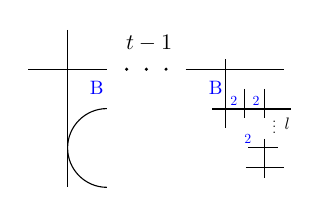
\begin{tikzpicture}[scale=0.5]
     \coordinate (C1) at (-1.50, 3.00);
  \coordinate (D1) at (-0.50, 3.00);
  \coordinate (A1) at (-1.00, 3.00);
  \coordinate (B1) at (-0.93, 3.26);

  \node[scale=0.8][above] at (B1) {$t-1$};
  \fill[black] (C1) circle (1.25pt);
  \fill[black] (D1) circle (1.25pt);
  \fill[black] (A1) circle (1.25pt);

  
  \coordinate (IIIrC) at (-4.00, 3.00);
  \coordinate (IIIrD) at (-2.00, 3.00);
  \coordinate (IIIrE) at (-3.00, 4.00);
  \coordinate (IIIrF) at (-3.00, 0.00);
  \coordinate (IIIrG) at (-2.00, 1.00);
  \coordinate (IIIrD_1) at (-2.26, 2.18);
  \draw (IIIrC) -- (IIIrD);
  \draw (IIIrE) -- (IIIrF);
  \draw (-2.00, 2.00) arc (90.0:270.0:1.00);
  \node[scale=0.7][above, text=blue] at (IIIrD_1) {B};


   \coordinate (G) at (0.76, 2.19);
  \coordinate (N) at (2.25, 1.25);
  \coordinate (O) at (2.58, 1.31);
  \coordinate (A) at (0.00, 3.00);
  \coordinate (B) at (2.50, 3.00);
  \coordinate (H) at (0.67, 1.99);
  \coordinate (I) at (2.67, 1.99);
  \coordinate (P) at (2.00, 1.23);
  \coordinate (Q) at (2.00, 0.23);
  \coordinate (R) at (1.59, 1.01);
  \coordinate (S) at (2.34, 1.01);
  \coordinate (T) at (1.53, 0.50);
  \coordinate (C) at (2.00, 2.50);
  \coordinate (D) at (2.00, 1.75);
  \coordinate (E) at (1.00, 3.25);
  \coordinate (F) at (1.00, 1.50);
  \coordinate (J) at (1.50, 2.50);
  \coordinate (K) at (1.50, 1.75);
  \coordinate (L) at (2.50, 0.50);
  \coordinate (M) at (1.22, 1.95);
  \coordinate (U) at (1.79, 1.95);
  \coordinate (V) at (1.58, 0.98);

  
  \node[scale=0.7][above, text=blue] at (G) {B};
  \node[scale=0.5][above] at (N) {$\vdots
$};
  \node[scale=0.6][above] at (O) {$l
$};
  \draw (A) -- (B);
  \draw (H) -- (I);
  \draw (P) -- (Q);
  \draw (R) -- (S);
  \draw (C) -- (D);
  \draw (E) -- (F);
  \draw (J) -- (J);
  \draw (J) -- (J);
  \draw (J) -- (K);
  \draw (T) -- (L);
  \node[scale=0.5][above, text=blue] at (M) {$2$};
  \node[scale=0.5][above, text=blue] at (U) {$2$};
  \node[scale=0.5][above, text=blue] at (V) {$2$};
\end{tikzpicture}% old pic:
% Namikawa--Ueno type: III-I_l-t
% Target MRNC type: III-I_l-t
% Adapted from Tim Dokchitser picture: I_{{\it n}}\e({\it m})III
% Parameter substitution: n -> l, m -> t
% \begin{tikzpicture}[xscale=0.57,yscale=0.62]
% \draw[thick,shorten >=2] (-0.09,0)--(3.67,0) node[inner sep=2pt,blue,above left,scale=0.8] {1};
% \draw[scale=0.8] (0,0) ++(0.05,0.3) node[anchor=east,blue,scale=0.7] {1} ++(0.3,-0.45)--++(115:0.75)++(295:0.15)++(245:0.15)--++(65:0.75)++(245:0.15)++(180:0.15)--++(0:0.22) ++(0:0.15) node{$\cdot$} ++(0:0.15) node{$\cdot$} node[above=0.1,anchor=south,scale=0.7]{$l$}++(0:0.15) node{$\cdot$} ++(0:0.15) --++(0:0.22)++(180:0.15)++(115:0.15)--++(295:0.75)++(115:0.15)++(65:0.15)--++(245:0.75)++(0.3,0.45) node[anchor=west,blue,scale=0.7] {1};\draw (2.44,0) 
 %    ++(0.06,-0.17)--++(-0.22,0.64)++(0.11,-0.24)  
 %    ++(0,0.02)
 %      node[blue,scale=0.7,inner sep=1,anchor=west]{1}
 %    ++(0,-0.02)
 %    ++(-0.16,0.02)--++(0.46,0.44)++(-0.12,0.08)  
 %    node{$\cdot$} ++(-0.06,0.16) node{$\cdot$}
 %    ++(-0.06,0.16) node{$\cdot$}++(0.17,-0.12)    node[auto,inner sep=5,scale=0.7,anchor=west]{$t$}
 %    ++(-0.25,0.23)--++(0.46,0.44)++(-0.19,0.04)   
  %   ++(0,-0.05)
  %     node[blue,scale=0.7,inner sep=1,anchor=east]{1}
  %   ++(0,0.05)
  %   ++(0.19,-0.04)++(-0.04,-0.2)--++(-0.22,0.64);
% \draw[thick,shorten >=2] (2.1,2)--(5.27,2) node[inner sep=2pt,blue,above left,scale=0.8] {4};
% \draw[shorten <=-3pt] (3.24,2)--node[inner sep=2pt,scale=0.8,blue,right] {1} (3.24,13/5);
% \draw[shorten <=-3pt] (4.04,2)--node[inner sep=2pt,scale=0.8,blue,right] {2} (4.04,13/5);
% \end{tikzpicture}


\end{document}
